\documentclass{article} 
\usepackage{amsmath} 
\usepackage{amssymb} 
\usepackage{amsthm} 
\usepackage[margin=0.2in]{geometry} 
\usepackage{hyperref} 
\usepackage{physics} 
\usepackage{tikz} 
\usepackage{mathtools}
\mathtoolsset{showonlyrefs} 
\theoremstyle{definition} 
\newtheorem{theorem}{Theorem}[section] 
\newtheorem{corollary}{Corollary}[theorem] 
\newtheorem{lemma}[theorem]{Lemma} 
\newtheorem{definition}{Definition}[section] 

\author{Connor Duncan}
\date{\today}
\title{Notes April 25}
\begin{document}
\maketitle


\subsection{Simple Pendulum}
Say we have some rigid body
\begin{center}
	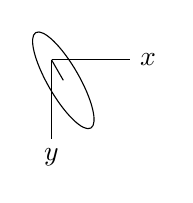
\begin{tikzpicture}
		\draw (0,0)--(1,0) node[anchor=west]{$x$};
		\draw (0,0)--(0,-1) node[anchor=north]{$y$};
		\draw[rotate=30] (0,-0.3) ellipse (0.2 and 0.7);
		\draw[rotate=30] (0,0)--(0,-0.3);
	\end{tikzpicture}
\end{center}
Small oscillations, we have
\begin{equation}
	\hat r=r(\hat y\cos(\theta+\varphi)+\hat x\sin(\theta+\varphi))
\end{equation}
and 
\begin{equation}
	\vec{v}=\dot\theta r\left[-\hat y\sin(\theta+\varphi)+\hat x\cos(\theta+\varphi)\right]
\end{equation}
then for $U$ we write
\begin{equation}
	U=mgd(1-\cos\theta)
\end{equation}
with 
\begin{align}
	E=\frac{1}{2}I\dot\theta^2+mgd(1-\cos\theta)
	\dot\theta=\pm\sqrt{\frac{2}{I}(E-mgd(1-\cos\theta)}
\end{align}
So we think about $1-\cos\theta=2\sin^2(\frac{\theta}{2})$. Let $\theta_0$ be the max value of $\theta$, i.e. where our approximation starts to fall apart.

To solve, we can evaluate
\begin{equation}
	T=\frac{2r_0}{\sqrt{gd}}\int_0^{\theta_0}\frac{d\theta}{\sqrt{\sin^2\frac{\theta_0}{2}-\sin^2\frac{\theta}{2}}}
\end{equation}
Let $k=\sin\frac{\theta_0}{2}$ and $k_z=\sin\frac{\theta}{2}$, so we write
\begin{equation}
	dz=\frac{1}{2}\frac{\cos\theta/2}{k}d\theta
\end{equation}
which makes 
\begin{equation}
	T=\frac{2r}{\sqrt{gd}}\int_{z=0}^1\frac{zkdz}{\sqrt{1-k^2z^2}}\frac{1}{k\sqrt{1-z^2}}
\end{equation}
in the small angle approxmation, we have 
\begin{equation}
	\sqrt{1-k^2z^2}\approx 1+\frac{1}{2}k^2z^2
\end{equation}
which allows us to break up $T$ into some shit that requires a lot of trig substitution, which ultimately yields
\begin{equation}
	T=\frac{4r_0}{\sqrt{gd}}\left(\frac{\pi}{2}+\frac{1}{2}k^2\frac{\pi}{4}\right)=\frac{2\pi r_0}{\sqrt{gd}}\left(1+\frac{1}{4}\sin^2\frac{\theta_0}{2}+\ldots\right)
\end{equation}
which gives us a term $T_0$ that tells us how much variation we have from the simple harmonic oscillator
\begin{equation}
	T_0=\frac{2\pi r_0}{\sqrt{gd}}
\end{equation}

For instance, if we plug in $\theta_0=23^\circ$, we get about a 1\% change.

Now, we do some
\subsubsection{Pertubation Theory}
and write down the ODE
\begin{equation}
	\ddot x+\omega_0^2x-\lambda x^2=0
\end{equation}
which, looking for $x(\lambda,t)$
\begin{equation}
x(\lambda,t)=x_0(t)+\lambda x_1(t)+\lambda^2 x_2(t)+\ldots
\end{equation}

\begin{align}
\dot x=\dot x_0+\lambda \dot x_1
\\
\ddot x=\ddot x_0+\lambda \ddot x_1
\end{align}
which gives
\begin{align}
	\ddot x+\omega_0^2x-\lambda x^2=0
	\\
	\ddot x_0+\lambda\ddot x_1+\omega_0^2(x_0+\lambda x_1)-\lambda(x_0+\lambda x_1)^2=0
	\\
	\ddot x_0+\lambda\ddot x_1+\lambda \ddot x_1+\omega_0^2\lambda x_1-\lambda x_0^2-2\lambda^2x_0x_1-\lambda^3x_1=0
\end{align}
first order perturbation of the thing, so if we're forcing it
\begin{equation}
\ddot x_1+\omega_0^2=A^2\cos^2\omega_0t
\end{equation}
So, what I think he did
\begin{equation}
	x(t)=x_0+\lambda x_1=_A\cos\omega_0 t-\lambda\frac{A^2}{6\omega_0^2}(\cos(2\omega_0 t)-3)
\end{equation}

3-wave coupling.

Kolomogorov (1941). No natural scale/boundary condition in hte problem

Imagine some eddy, that you've just broken up
\begin{center}
	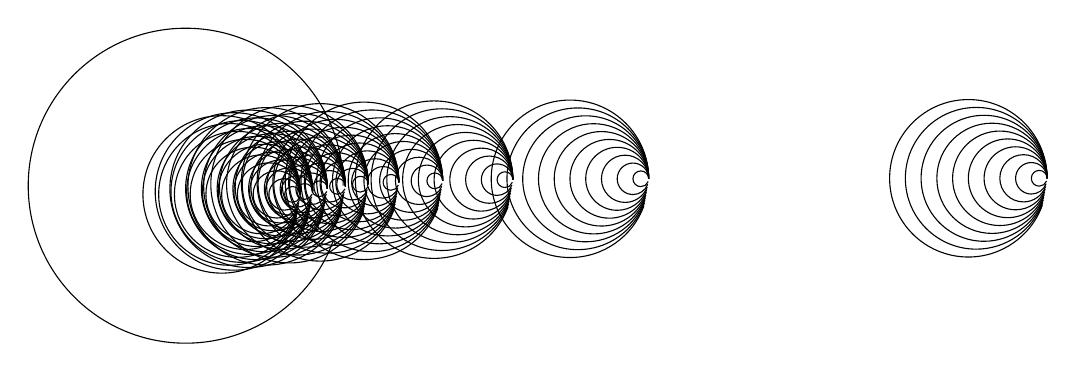
\begin{tikzpicture}
		\draw[->] (1,1) arc (0:340:2);
		\foreach \scale in {0.1,0.2,...,1}
		{
			\foreach \x in {0.1,0.2,...,1}
			{
				\draw ({1/\x*cos(10*2*3.14159*\x)},{1/\x*sin(10*2*3.14159*\x)}) arc (0:340:\scale);
				}
			}
	\end{tikzpicture}
\end{center}
<++>
\end{document}
